% ~~~ [ Profiling ] ~~~~~~~~~~~~~~~~~~~~~~~~~~~~~~~~~~~~~~~~~~~~~~~~~~~~~~~~~~~~

\subsubsection{Profiling}
\label{sec:ver_profiling}

The initial implementation of the LLVM IR library (see section \ref{sec:impl_llvm_ir_library}) focused on correctness, and strived to be as simple and straight forward as possible. Once feature complete and thoroughly tested, the library was profiled for the first time and a major performance bottleneck was discovered; as illustrated in figure \ref{fig:lexer_pprof}. When scanning letters (e.g. \texttt{lexLetter}), the lexer used a hash map to check if the scanned letters were part of a keyword. As letter make up the majority of the characters in LLVM IR source files, this caused an extensive use of hash map iterations which accounted for roughly 70\% of the total execution time. To fix this issue, a benchmark test was implemented to measure the performance changes between the original and the updated version; as further described in section \ref{sec:ver_benchmarks}. At this stage, only CPU profiling has been utilized and memory profiling has been deferred to future performance work.

\begin{figure}[htbp]
	\begin{center}
		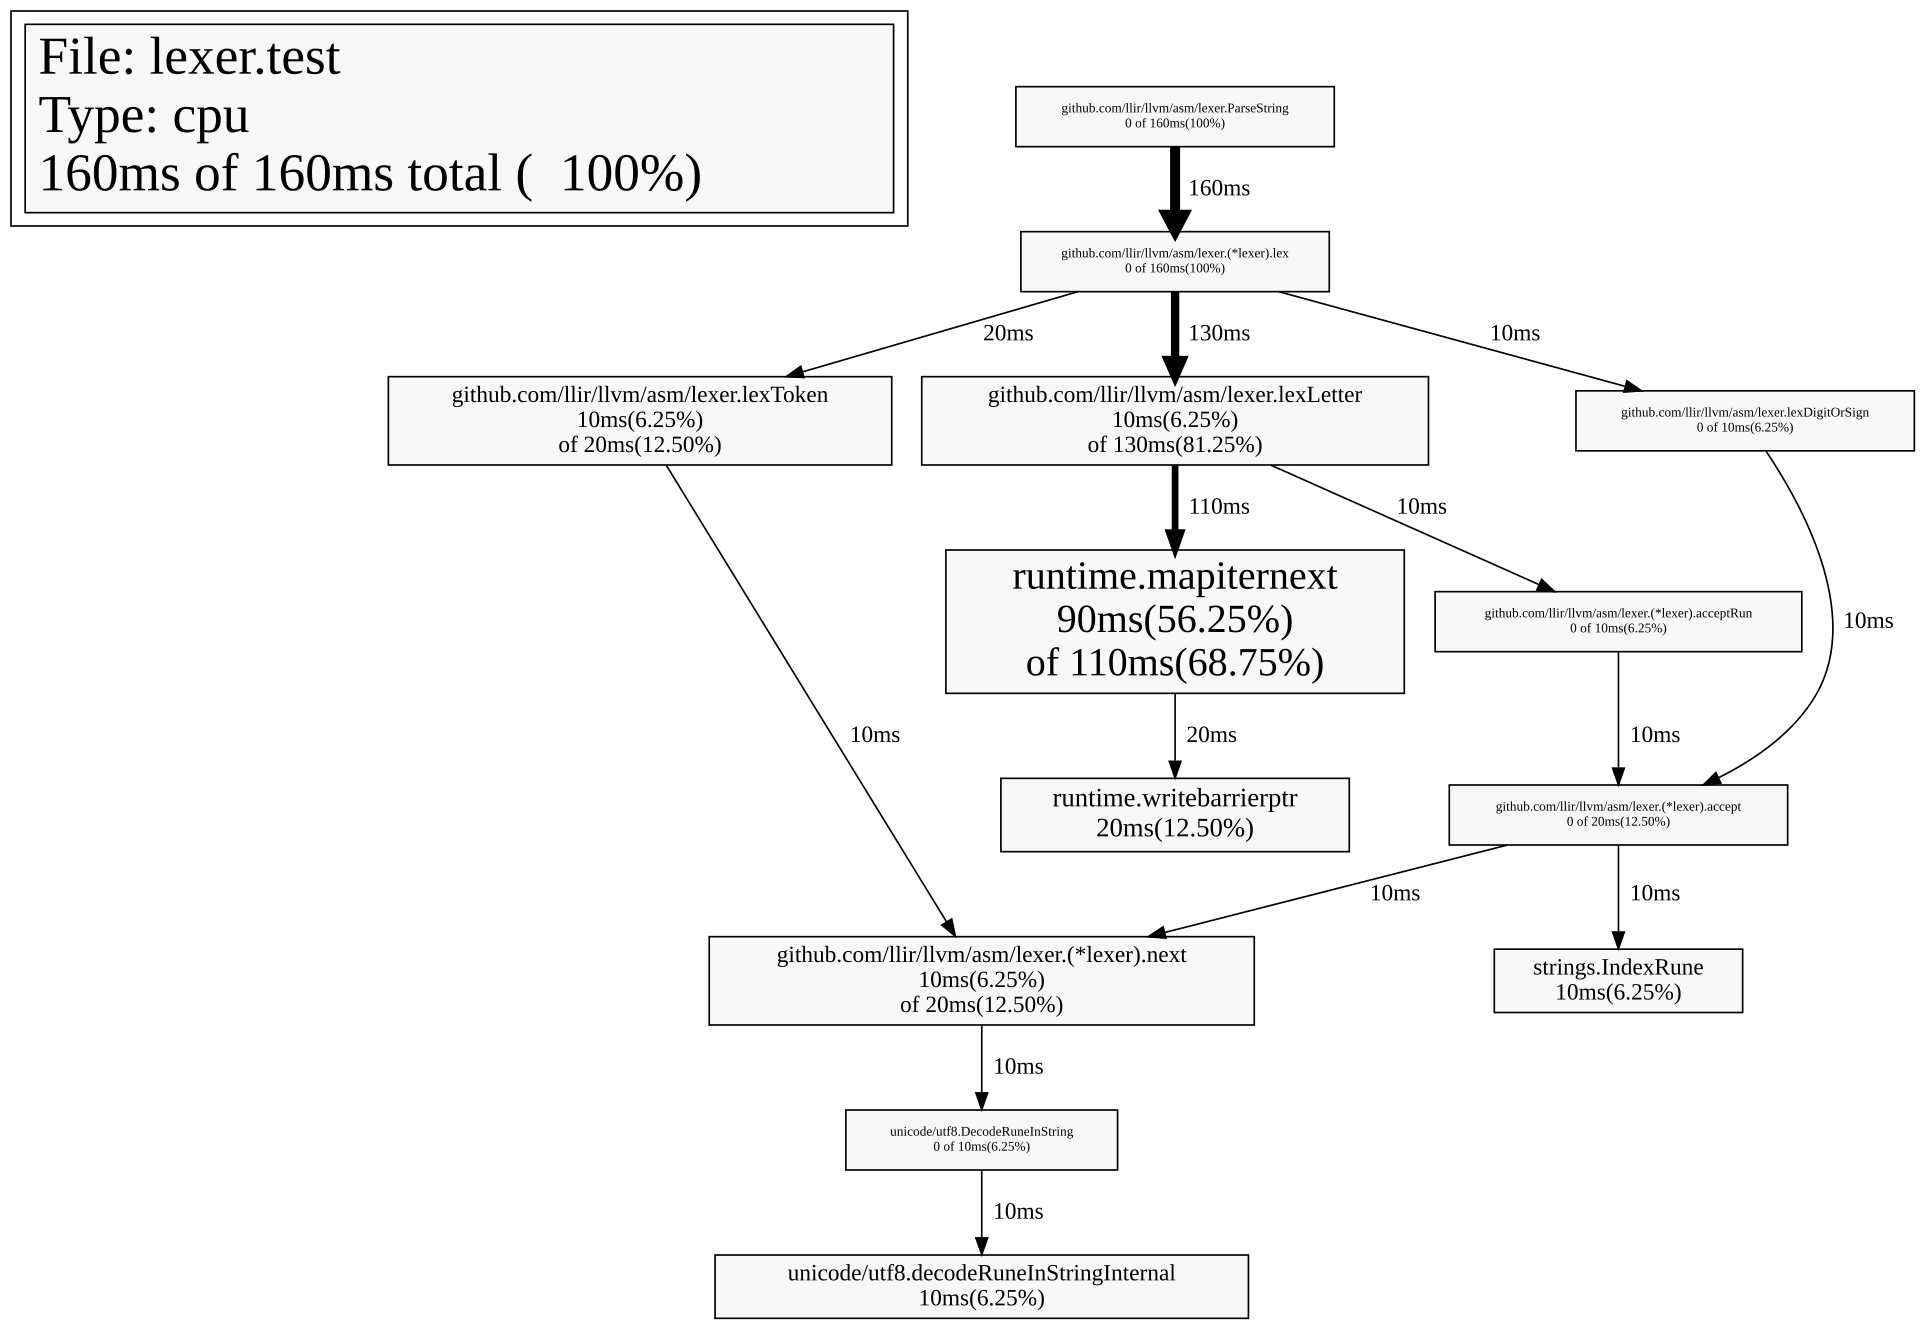
\includegraphics[width=\textwidth]{inc/8_ver/lexer_pprof.png}
		\caption{A major performance bottleneck was located when profiling the LLVM lexer library for the first time. Roughly 70\% of the total execution time was spent doing hash map iterations (i.e. \texttt{runtime.mapiternext}).}
		\label{fig:lexer_pprof}
	\end{center}
\end{figure}
